\section*{Introduction}

% MOTIVATION
\begin{frame}[noframenumbering,c]
	\begin{overprint}
				
		\onslide<1>
			\vskip2.75ex
			\begin{figure}[htp]
				\centering
				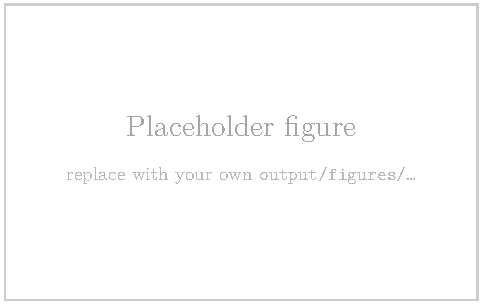
\includegraphics[width=2in]{../../assets/placeholders/placeholder-figure.pdf}
			\end{figure}		

		\onslide<2>
			\vskip2.75ex
			\begin{figure}[htp]
				\centering
				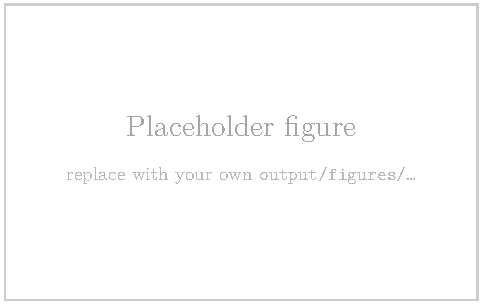
\includegraphics[width=2in]{../../assets/placeholders/placeholder-figure.pdf}
			\end{figure}											

	\end{overprint}		
\end{frame}

% THIS PAPER
\begin{frame}{This paper}
	\blockhead*{Motivation}
	\begin{itemize}
		\item Many people have ``an'' idea of North
		\item But little real experiences of it
	\end{itemize}

	\blockhead{Question}
	\begin{itemize}
		\item What is living in the North actually like?
		\begin{itemize}
			\item Some point
			\item Another point
		\end{itemize}
		\item Where does the idea of North start and end?
	\end{itemize}

	\blockhead{Approach}
	\begin{itemize}
		\item Interview five people who have had direct exposures to the North
		\item Build and estimate model of Northern migration
	\end{itemize}
\end{frame}


% THIS PAPER
\begin{frame}{Preview of findings}
	\begin{enumerate}
		\setlength\itemsep{\slideitemgap}
		\item Finding 1
		\item Finding 2
		\item Finding 3
	\end{enumerate}
\end{frame}
